\subsection{Generierung von Dateien}\label{subsec:generierung-von-dateien}
Aus einer workflow beschreibung können bis zu fünf verschiedene Typen von Dateien generiert werden.
Der Einstiegspunkt und somit der Start des Parsens und der Generierung ist die \textit{BoardGenerator}-Klasse.
Diese hat Methoden um Eingaben entweder von einer Datei oder eines Strings weiterzuverarbeiten.
Nachdem mittels des Parsers aus der Eingabe ein fertiges Board-Objekt erstellt wurde, werden weitere Klassen zur Generierung verwendet.
HTML-Dateien werden vom HtmlGenerator generiert, hierbei handelt es sich um Mockups und das Event Storming Board.
Mockups können allerdings auch als FXML-Datei generiert werden, um eine Grundlage für eine JavaFx-Anwendung zu bilden, diese Generierung
übernimmt der FxmlGenerator.
Zuletzt vereint der DiagramGenerator die Generierung von Objekt- und Klassendiagrammen.
Außer der \textit{BoardGenerator}-Klasse sind die restlichen Generator-Klassen für die Vorbereitung der Daten zuständig.
Diese erhalten Eingaben von dem BoardGenerator, bereiten diese Eingabe auf, je nachdem welche Daten benötigt werden und enthalten eine
separate Methode zum Erstellen von Dateien im Dateisystem.
Das Bauen einer Datei in Form eines Strings wird in einer gesonderten \textit{Constructor}-Klasse erledigt.
Da es fünf verschiedene Typen von Dateien gibt und das Bauen für jede Datei anders ist, existieren fünf \textit{Constructor}-Klassen, für jeden Dateityp eine.
Im Folgenden werden die Aufbereitungsschritte genauer beleuchtet.

\subsubsection{Event Storming Board}
Für die Generierung des Event Storming Boards bedarf es keiner Bearbeitung des HtmlGenerators, da das gesamte Board generiert werden soll und die Daten,
welche vom Parser erstellt wurden bereits optimiert sind.
Die HTML-Datei wird mittels StringTemplates, welche in einer StringTemplateGroup organisiert sind, zusammengebaut.
Für jeden workflow im Board-Objekt wird eine neue Reihe in der HTML-Datei angelegt.
Innerhalb einer workflow-Reihe werden alle dazugehörigen Notes gebaut.
Hierbei wird zwischen den verschiedenen Notes unterschieden, um verschiedene Darstellungen zu ermöglichen.
Je nach Note wird eines von drei StringTemplates verwendet.
Für die Standard-Notes wird lediglich eine neue \textit{Card}, eine Bootstrap CSS-Klasse, erstellt, welche den Typen des Notes, dessen Content und eine bestimmte Farbe übergeben bekommt.
Für die organisatorischen Notes, User, Service und ExternalSystem wird eine Card erstellt, welche kleiner als die eines normalen Notes ist.
Zudem wird in organisatorischen Notes nur ein Icon und der Bezeichner angezeigt, wobei das Icon ein Bootstrap Icon ist.
Data- und Page-Notes werden gesondert mit einem dritten StringTemplate behandelt, da es neben Typ, Content und Farbe noch einen Link gibt, welcher als Button definiert und für die Verwendung
im WebEditor genutzt wird.

\begin{figure}[h]
    \centering
    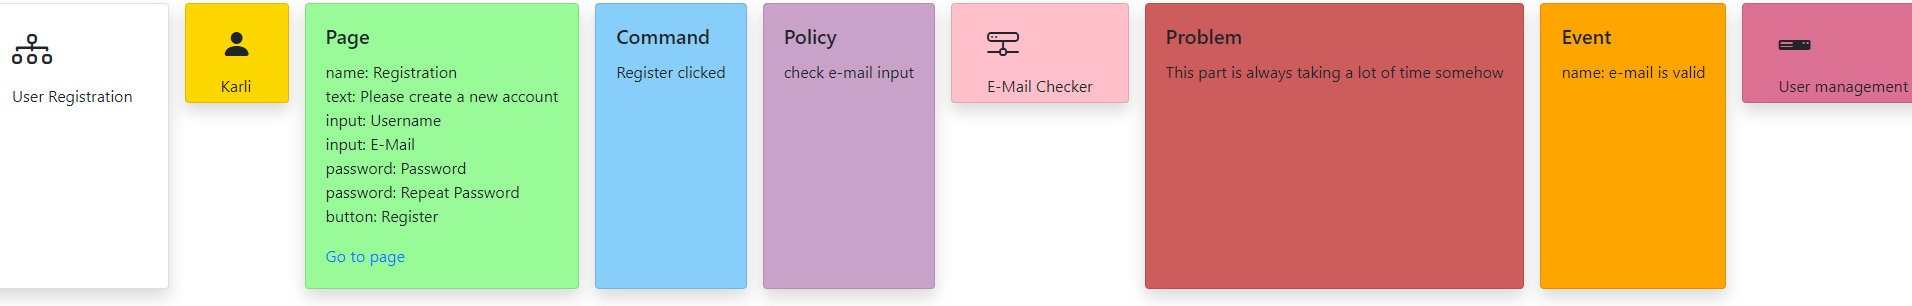
\includegraphics[width=1.0\textwidth]{images/3.1/board}
    \caption{Mittels fulibWorkflows generiertes Event Storming Board}
    \label{fig:generated-board}
\end{figure}

In Abbildung~\ref{fig:generated-board} ist ein Ausschnitt des in Listing~\ref{listing:workflowNotes} beschriebenen Workflows in
Form eines generierten Event Storming Boards dargestellt.
Hierbei sind die zuvor beschriebenen Unterschiede zwischen den verschiedenen Notes erkennbar.
Jeder Note-Typ besitzt eine eigene Farbe, wobei für User, Service und ExternalSystem eine kleinere Card und jeweils ein
eigenes Icon erkennbar sind.
Ebenfalls ist der Page-Note der Note mit den meisten Informationen in diesem Ausschnitt, da nur dort zusätzliche Informationen
in der Workflowbeschreibung existierten.

\subsubsection{Mockups HTML/FXML}
\todo{STG für Mockups Html und fxml mit Bildern}

\subsubsection{Objektdiagramme}
\todo{STG für Objekte, Fulib Notation zum generien mit FulibTools mit Bildern}

\subsubsection{Klassendiagramme}
\todo{Wie wird aus allen Objekten ein Klassendiagramm? Aufbauen eine neuen Klassenmodells mittels fulib und dann fulibtools zur generierung mit Bildern}
